
\begin{figure}
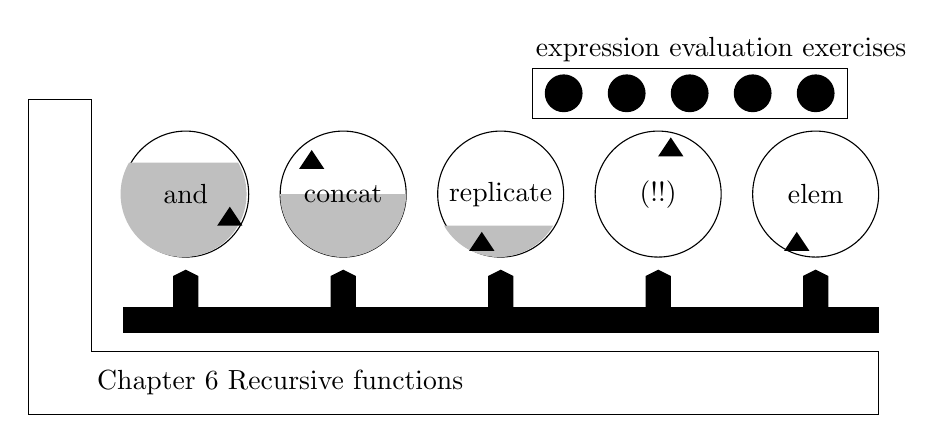
\begin{tikzpicture}[scale=0.08]

\foreach \x in {25,50,75,100,125}
     \draw (\x ,35) circle(10);
\node (sm) at (40,5) {Chapter 6 Recursive functions};
\fill[lightgray] (16,40) arc [start angle=150,   delta angle=240,
				x radius=10, y radius=10, color=lightgrey] -- cycle;
\node (o1) at (25,35) {and};
\fill[lightgray] (40,35) arc [start angle=180,   delta angle=180,
				x radius=10, y radius=10, color=lightgrey] -- cycle;
\node (o2) at (50,35) {concat};
\fill[lightgray] (66,30) arc [start angle=210,   delta angle=120,
				x radius=10, y radius=10, color=lightgrey] -- cycle;
\node (o3) at (75,35) {replicate};
\node (o4) at (100,35) {(!!)};
\node (o5) at (125,35) {elem};
\fill[black] (15,13) rectangle (135,17);
\foreach \x in {23,48,73,98, 123}
      \fill[black] (\x,17) -- (\x,22) -- (\x+2,23) -- (\x+4, 22) -- (\x+4,17) -- cycle;

\draw  (80,47) rectangle (130,55);
\foreach \x in {85,95,105, 115, 125}
\fill[black] (\x ,51) circle(3);
\node (eqr) at (110,58) {expression evaluation exercises}; 
\draw (0,0) -- (0,50) -- (10,50) -- (10,10) -- (135,10) -- (135,0) -- cycle;

\fill[black]  (30,30) -- (34,30) -- (32,33) -- cycle;
\fill[black]  (43,39) -- (47,39) -- (45,42) -- cycle;
\fill[black]  (70,26) -- (74,26) -- (72,29) -- cycle;
\fill[black]  (100,41) -- (104,41) -- (102,44) -- cycle;
\fill[black]  (120,26) -- (124,26) -- (122,29) -- cycle;


\end{tikzpicture}
\caption{Task class Recursive functions}\label{fig:taskclasserecursive}
\end{figure}


